\subsection{Indicator Layer Subsystems}
The indicator layer will be responsible for the output of the system, where the indicator subsystem
consists of an industrial light tower, which displays the status of the working cell.

\begin{figure}[h!]
	\centering
 	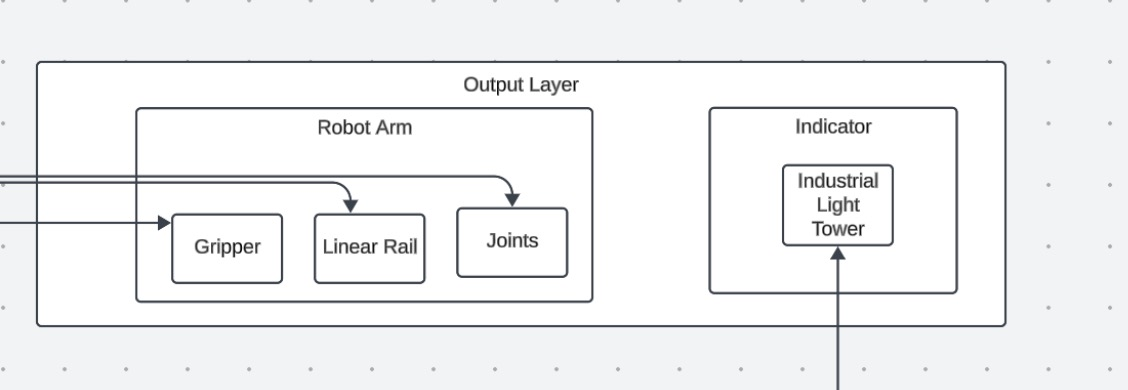
\includegraphics[width=0.60\textwidth]{images/indicator.jpg}
 \caption{Indicator Layer Subsystem}
\end{figure}

\subsubsection{Industrial Light Tower}
An industrial light tower system, typically used in a working cell or industrial setting, serves several
essential responsibilities to ensure the efficient and safe operation of the workspace. The specific responsibilities of an industrial light tower system may vary depending on the application. For our system,
it serves as an inference to the work environment as it indicates different modes with colored LEDs as
get input from the controller and outputs as LEDs.

\subsubsection{Subsystem Operating System}
No operating system required. 

\subsubsection{Subsystem Software Dependencies}
No software dependencies required by the subsystem.

\subsubsection{Subsystem Programming Languages}
No programming Language required.

\subsubsection{Subsystem Data Structures}
No data structures required. 

\subsubsection{Subsystem Data Processing}
No data processing require.


